\section{Problem prevođenja}\label{ch:analiza}

Analizom postojećih alata za upravljanje prevodima mogu se uočiti prednosti i mane tih alata. 
Zadatak analize postojećih sistema je upoznavanje sa problematikom kako bi se izbegle greške
koje su ti sistemi napravili, ali i prikupljanje dobrih ideja i funkcionalnosti koje pružaju ti sistemi.


\subsection{Postojeća okruženja}\label{sec:analiza-postojeca_okruzenja}

Na tržištu postoji dosta rešenja koji se bave upravljanjem prevodima. Jedno od takvih rešenja je 
\textit{BabelEdit}~\cite{BabelEdit}, editor prevoda za veb aplikacije. Program se instalira na klijentskom računaru.
Program podržava pravljenje projekta u koji se kasnije uvoze fajlovi sa prevodima. Kada korisnik završi 
sa prevođenjem, može da izveze prevode iz projekata u razne formate. Ovaj alat ne nudi mogućnost kolaboracije,
a fajlovi se nalaze na lokalnom računaru, i kao takav je pogodan jedino za manje projekte. Ovaj alat ima 
probni period od nekoliko dana, a kasnije se mora platiti.

\begin{figure}[h]
    \centering
    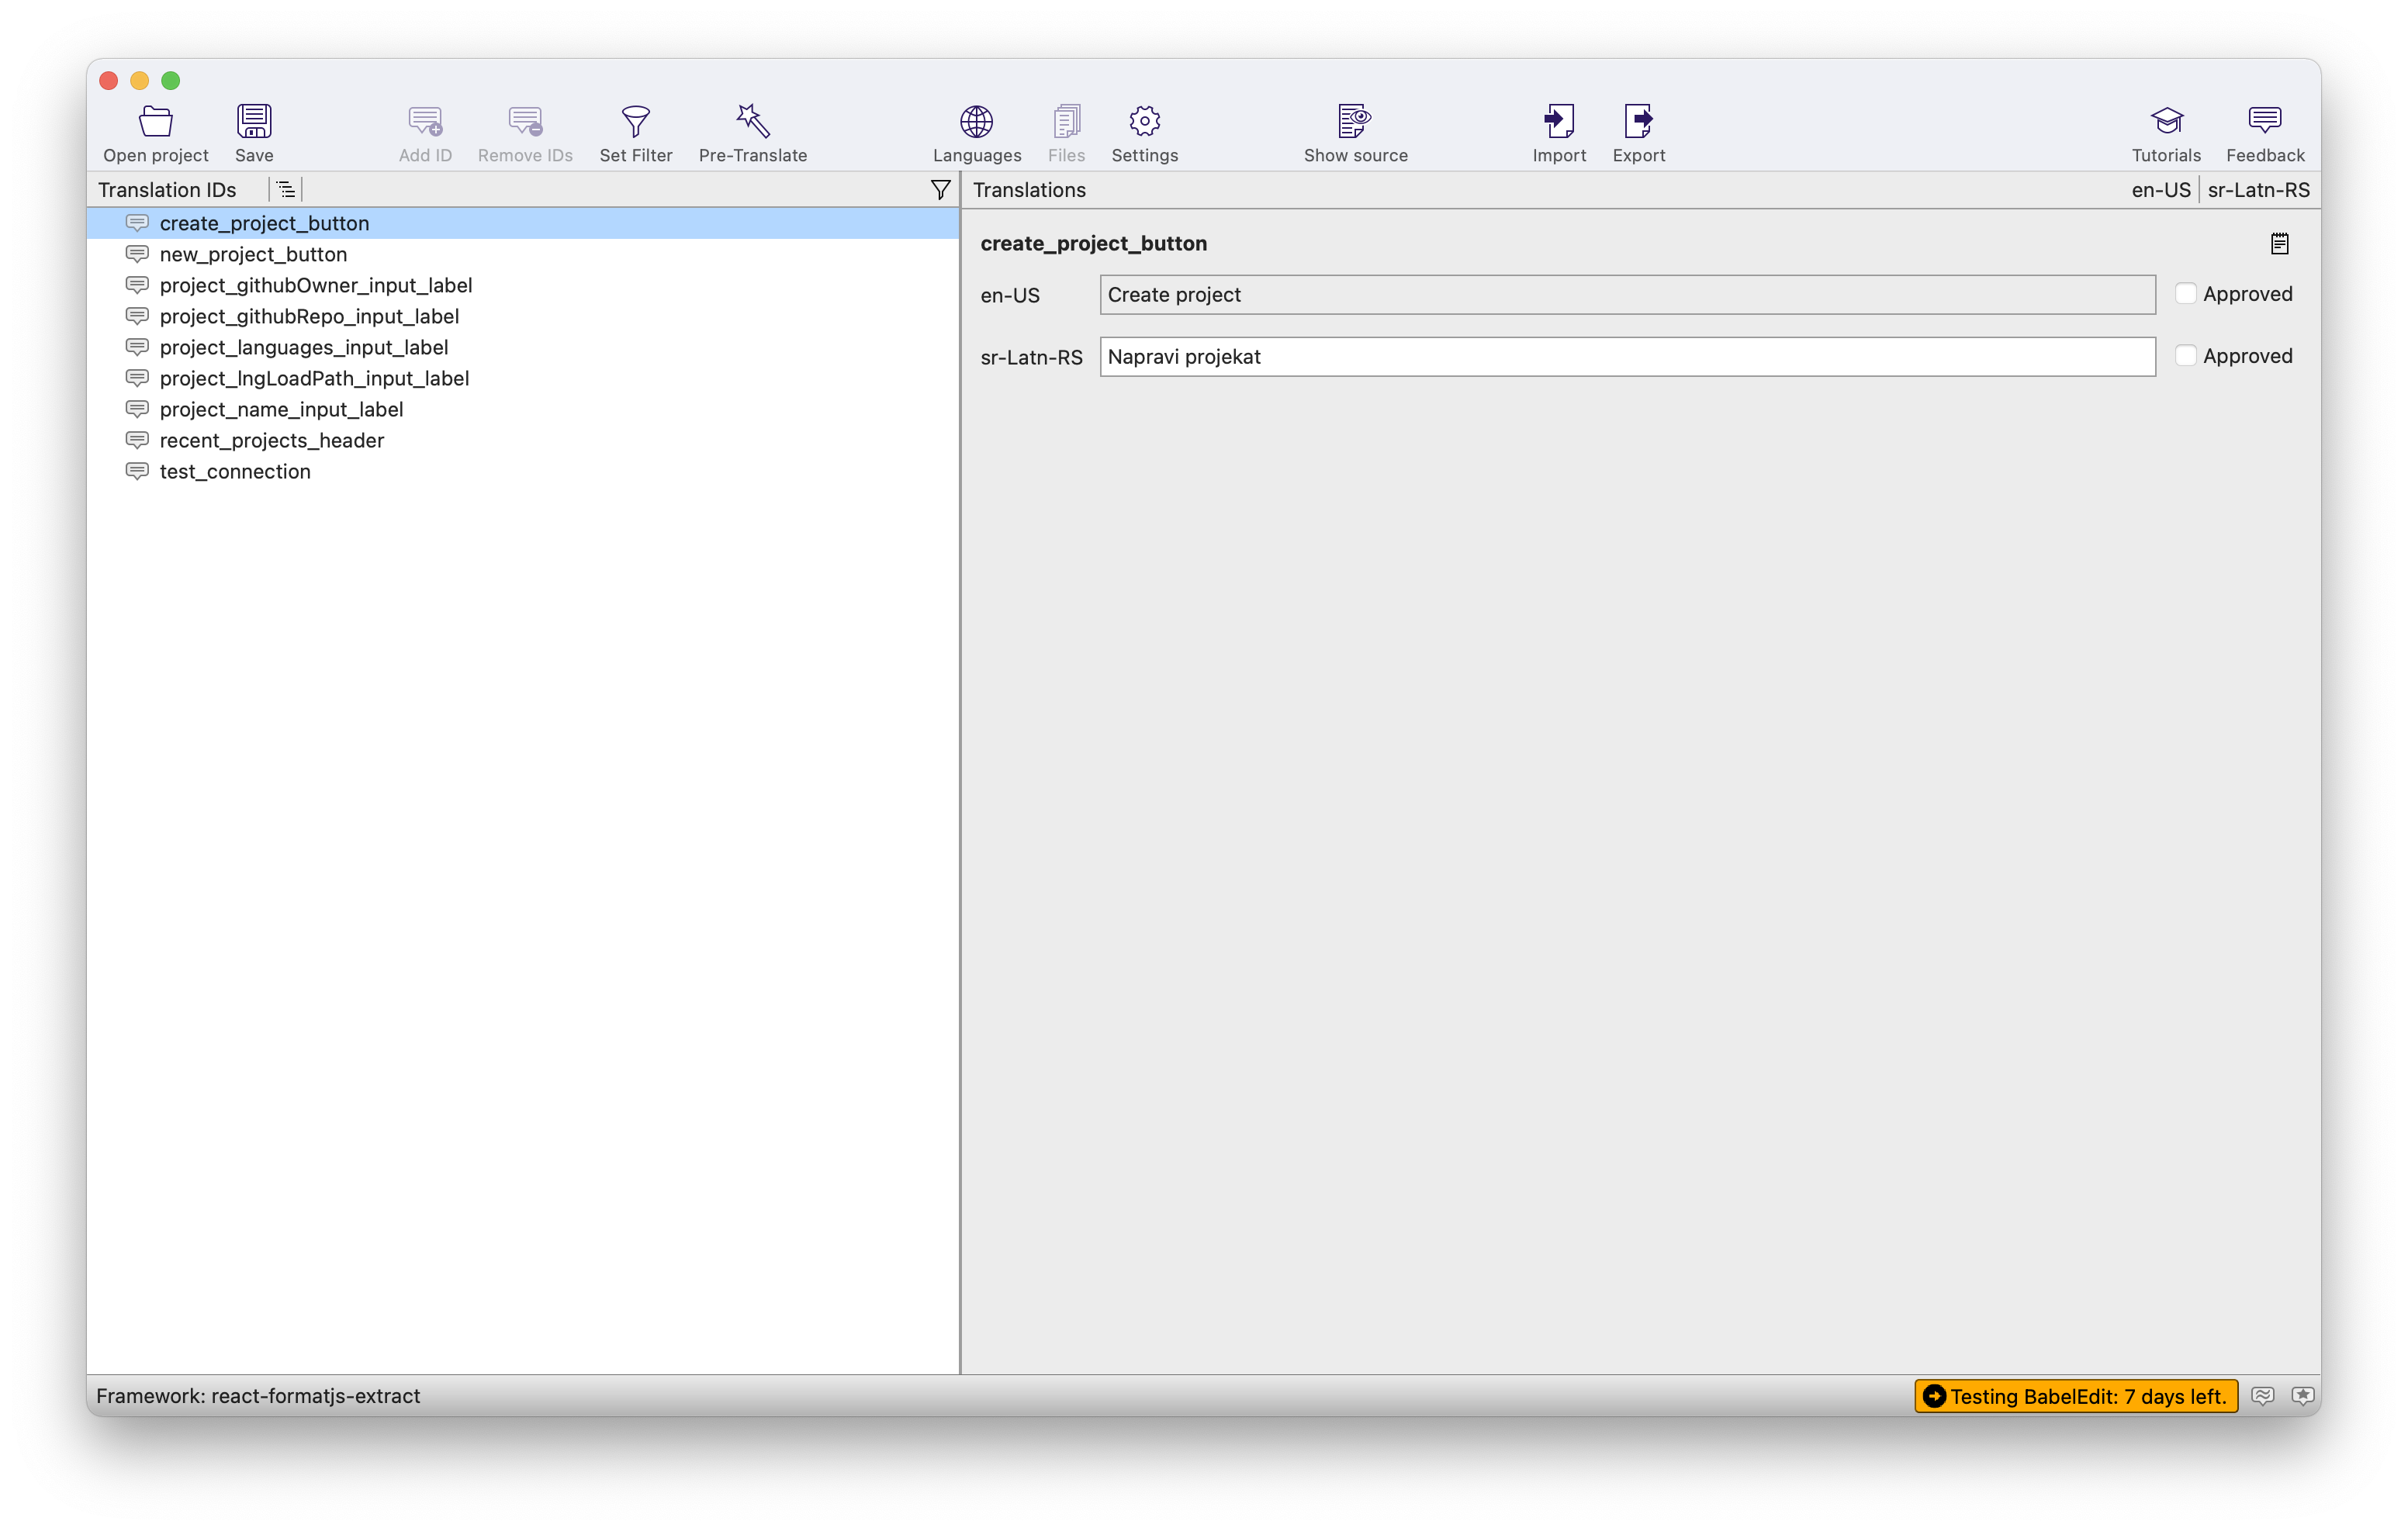
\includegraphics[width=1\textwidth]{babeledit}
    \caption{Korisnički interfejs alata \textit{BabelEdit}}
\end{figure}

Drugo popularno rešenje je \textit{Localazy}~\cite{Localazy}, platforma koja podržava više od 50 radnih okvira, 
formata fajlova. Platforma se nalazi u oblaku i pristupa joj se preko veb pregledača. Na platformi se može 
napraviti novi projekat u okviru kojeg se mogu uvesti fajlovi sa prevodima za izabrani jezik. Istom projektu 
može pristupiti više prevodilaca i uređivati prevode. Kada se izabere fajl za prevod, sa leve strane se može 
videti ključ za nisku koju treba prevesti, a pored njega i sam prevod. Prevodi su kasnije dostupni preko 
mreže za dostavu sadržaja (eng. \textit{Content Delivery Network, CDN}). \textit{Localazy} omogućava besplatno korišćenje za 
projekte koji imaju najviše 200 ključeva, što odlikuje manje projekte.

\begin{figure}[h]
    \centering
    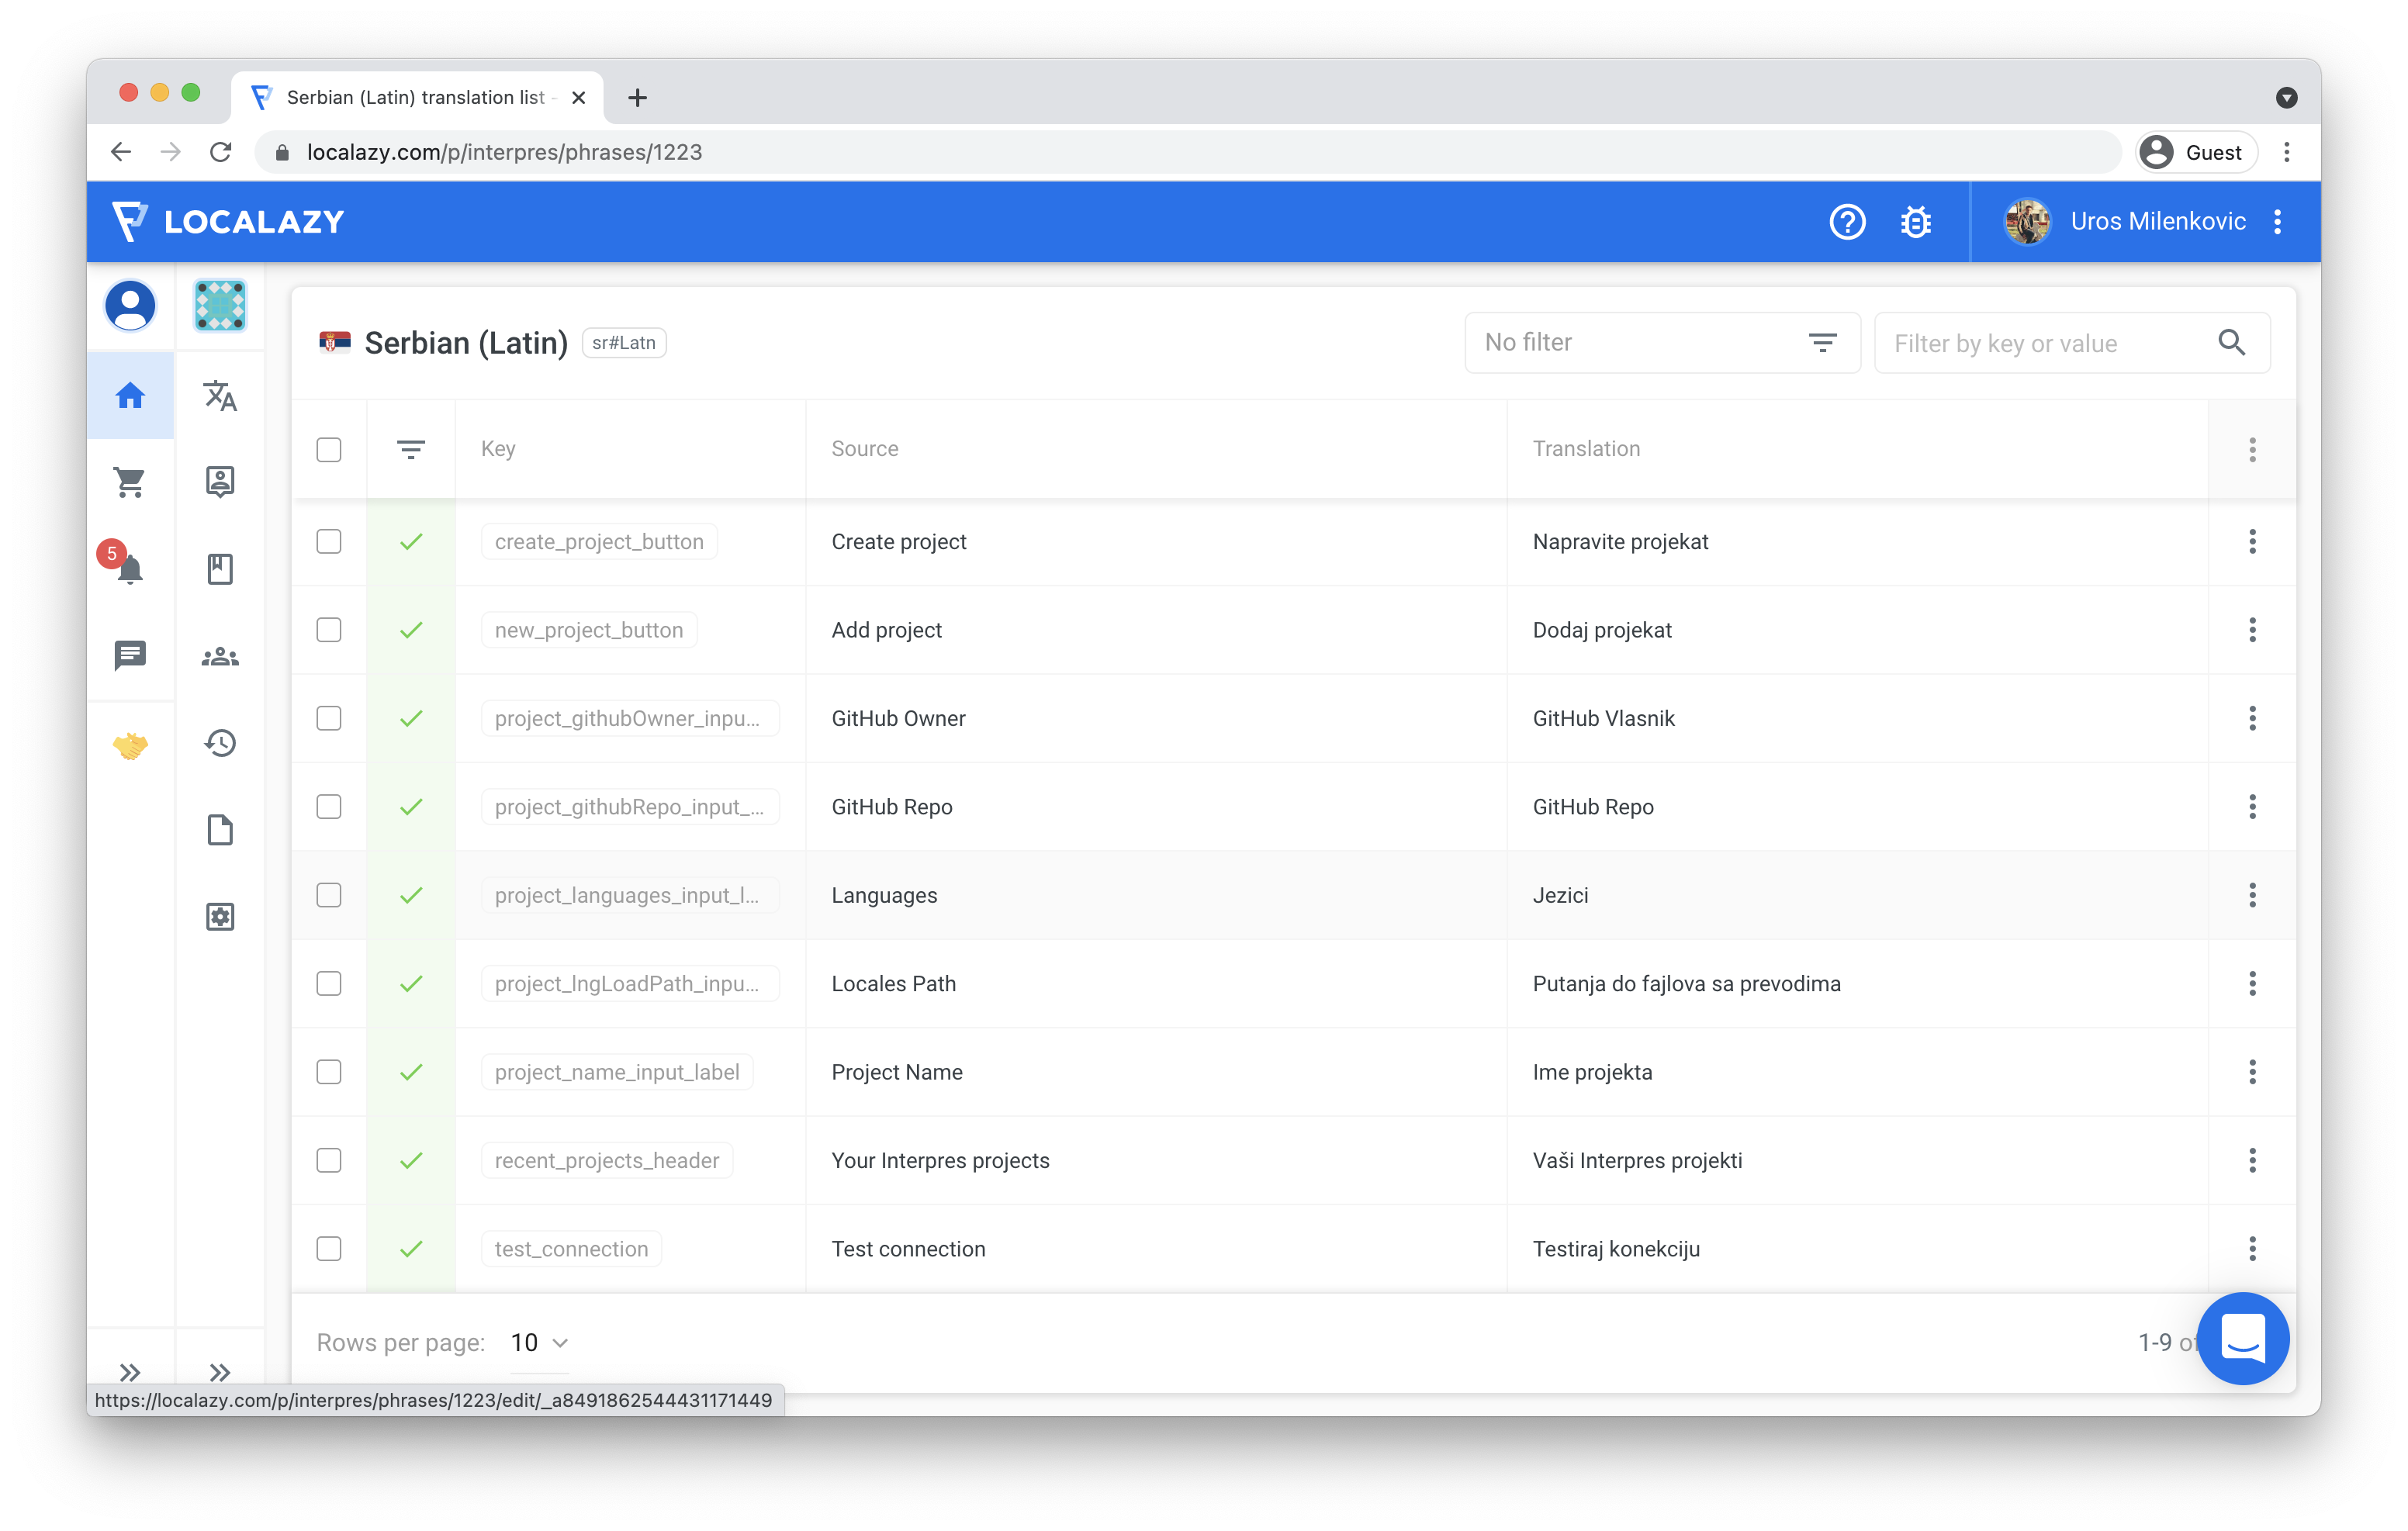
\includegraphics[width=1\textwidth]{localazy}
    \caption{Korisnički interfejs alata \textit{Localazy}}
\end{figure}

Navedeni alati poseduju i integraciju sa sistemima za mašinsko prevođenje, što u mnogome olakšava posao 
prevodiocima. Svakako, na kraju je potrebna provera od strane čoveka kako bi sadržaj bio u većoj meri prilagođen. 

\subsection{Moguća unapređenja}\label{sec:analiza-moguca_unapredjenja}

Oba analizirana alata pružaju nekakav oblik obaveštenja da je prevodilac završio sa poslom. U slučaju alata \textit{BabelEdit}
potrebno je da prevodilac izveze prevode i kasnije izvezene fajlove da pošalje programeru. Kod \textit{Localazy} 
je proces malo bolji jer prevodilac ne treba da šalje nikakve fajlove, već samo da obavesti programera, 
koji će ih kasnije preuzeti sa \textit{CDN}.

Ovde se može primetiti da je moguće automatizovati proces predaje prevoda. Potrebno je samo da klikom dugmeta
prevodilac obavesti sistem da je završio svoj posao. Ta akcija bi trebalo da pokrene izgradnju nove verzije aplikacije.